%========================
% Document class and theme
%========================
\documentclass[8pt]{beamer}
\usetheme[progressbar=frametitle]{metropolis}
\setbeamersize{text margin left=10mm, text margin right=10mm}
\usepackage{appendixnumberbeamer} % appendix slide numbering
\setbeamertemplate{theorems}[numbered]

%========================
% Core packages
%========================
\usepackage{amsmath, amsfonts, amssymb, amsthm} % math + theorems
\usepackage{booktabs}        % professional tables
\usepackage{hyperref}        % hyperlinks
\usepackage{xcolor}          % colors
\usepackage{xspace}          % spacing for custom commands

%========================
% Algorithms
%========================
\usepackage{algorithm}
\usepackage{algpseudocode}
\newtheorem{proposition}{Proposition}
\usepackage{bbm}

%========================
% Plots and TikZ
%========================
\usepackage{pgfplots}
\usepgfplotslibrary{dateplot}
\usepackage{tikz}
\usetikzlibrary{positioning}

%========================
% Listings (code)
%========================
\usepackage{listings}
\lstset{
    basicstyle=\ttfamily\small,
    breaklines=true,
    numbers=left,
    numberstyle=\tiny
}

% R style
\lstdefinelanguage{R}{
  morekeywords={TRUE,FALSE},
  deletekeywords={data,frame,length,as,character},
  otherkeywords={0,1,2,3,4,5,6,7,8,9},
  keywordstyle=\color{blue},
  commentstyle=\color{DarkGreen},
  stringstyle=\color{DarkGreen},
  basicstyle=\ttfamily\small
}

% Python style
\lstdefinelanguage{PythonCustom}{
  language=Python,
  keywordstyle=\color{blue},
  commentstyle=\color{gray},
  stringstyle=\color{red},
  basicstyle=\ttfamily\small
}

%========================
% Custom commands
%========================
\newcommand{\themename}{\textbf{\textsc{metropolis}}\xspace}

%========================
% Custom footline
%========================
\setbeamertemplate{footline}
{%
  \leavevmode%
  \hbox{%
  \begin{beamercolorbox}[wd=.35\paperwidth,ht=2.5ex,dp=1.5ex,center]{author in head/foot}%
    \usebeamerfont{author in head/foot}\insertshortauthor
  \end{beamercolorbox}%
  \begin{beamercolorbox}[wd=.3\paperwidth,ht=2.5ex,dp=1ex,center]{title in head/foot}%
    \usebeamerfont{title in head/foot}\insertshorttitle
  \end{beamercolorbox}%
  \begin{beamercolorbox}[wd=.3\paperwidth,ht=2.5ex,dp=1ex,right]{date in head/foot}%
    \usebeamerfont{date in head/foot}\insertframenumber{} / \inserttotalframenumber
  \end{beamercolorbox}}%
  \vskip0pt%
}

%========================
% Beamer tweaks
%========================
\setbeamertemplate{navigation symbols}{} % remove default navigation symbols


\title{Chapter 4}
\subtitle{Markov Chain Monte Carlo. \\ Metropolis-Hastings Algorithm.}
\author{Ali Raisolsadat}
\institute{School of Mathematical and Computational Sciences \\ University of Prince Edward Island}
\date{}

%========================
% Begin document
%========================
\begin{document}

%-------------------
% Title frame
%-------------------
\maketitle

%--------------------------------------------
% Slide 1: Introduction to Metropolis–Hastings
%--------------------------------------------
\begin{frame}{Metropolis–Hastings}
The Metropolis algorithm is a special case of the more general \alert{Metropolis–Hastings} algorithm.

\begin{itemize}
    \item Metropolis-Hastings uses a general \alert{proposal distribution}
    \[
    	q(\hat{x}^{(t+1)} \mid x^{(t)}) = q(x^{(t)} \rightarrow \hat{x}^{(t+1)})
    \]
    \item In the Metropolis algorithm, $q$ is typically a symmetric Gaussian centered at $x^{(t)}$.
\end{itemize}

MH accepts the proposed state $\hat{x}^{(t)}$ with probability
\[
\frac{\tilde{p}(\hat{x}^{(t)})}{\tilde{p}(x^{(t-1)})} \cdot \frac{q(x^{(t-1)} \rightarrow \hat{x}^{(t)})}{q(\hat{x}^{(t)} \rightarrow x^{(t-1)})}
\]

The ratio
\[
    \frac{q(x^{(t-1)} \rightarrow \hat{x}^{(t)})}{
          q(\hat{x}^{(t)} \rightarrow x^{(t-1)})}
\]
ensures \alert{detailed balance} when the proposal is asymmetric: if a move is easier to propose one way than the reverse, it becomes harder to accept.

Under mild conditions (e.g., $q(x \rightarrow x') > 0$ for all states), the Markov chain converges to the target distribution. However, the \alert{rate of convergence} can vary significantly depending on the choice of $q$.
\end{frame}

%--------------------------------------------
% Slide 2: Metropolis–Hastings Example
%--------------------------------------------
\begin{frame}{Metropolis–Hastings Example: Rolling a Die with Coins}
Suppose we want to \alert{sample from a fair 6-sided die}:
\[
    P(X = c) = \frac{1}{6} \qquad c \in \{1,\dots,6\}
\]
but we have no die or computer. We only have \alert{coins}. We also want to avoid rejection sampling.

Consider the following \alert{random-walk proposal} on $\{1,\dots,6\}$:
\begin{itemize}
    \item If $x = 1$, always propose $2$
    \item If $x = 2$, propose $1$ or $3$ with probability $1/2$ each
    \item If $x = 3$, propose $2$ or $4$ with probability $1/2$ each
    \item If $x = 4$, propose $3$ or $5$ with probability $1/2$ each
    \item If $x = 5$, propose $4$ or $6$ with probability $1/2$ each
    \item If $x = 6$, always propose $5$
\end{itemize}

What are we doing? flip a coin; move up on heads (if possible), move down on tails (if possible).  
This induces a \alert{random walk} on the state graph.

\centering
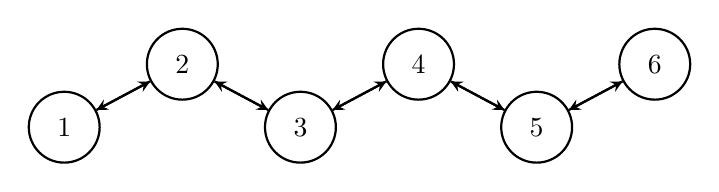
\begin{tikzpicture}[>=stealth,thick]

\tikzstyle{state}=[circle,draw,minimum size=0.9cm]

\node[state] (1) at (0,0) {1};
\node[state] (2) at (1.5,0.8) {2};
\node[state] (3) at (3,0) {3};
\node[state] (4) at (4.5,0.8) {4};
\node[state] (5) at (6,0) {5};
\node[state] (6) at (7.5,0.8) {6};

\foreach \a/\b in {1/2,2/3,3/4,4/5,5/6}
    \draw[->] (\a) -- (\b);

\foreach \a/\b in {2/1,3/2,4/3,5/4,6/5}
    \draw[->] (\a) -- (\b);

\end{tikzpicture}
\end{frame}

%--------------------------------------------
% Slide 3: Metropolis–Hastings Example
%--------------------------------------------
\begin{frame}{Metropolis–Hastings Example: Rolling a Die with Coins}

“Roll a die with a coin’’ by using the \alert{random-walk proposal $q$} in M-H:
\[
q(1 \rightarrow 2) = 1,\quad 
q(2 \rightarrow 1) = \tfrac{1}{2},\quad 
q(2 \rightarrow 3) = \tfrac{1}{2},\; \dots,\;
q(6 \rightarrow 5) = 1
\]

If $x = 3$ and we propose $\hat{x} = 2$, we always accept. The acceptance check is
\[
u < \frac{p(2)}{p(3)}
    \cdot
    \frac{q(2 \rightarrow 3)}{q(3 \rightarrow 2)}
  = \frac{1/6}{1/6} \cdot \frac{1/2}{1/2}
  = 1
\]

The same holds for any $x$ in the “middle’’ states $\{2,3,4,5\}$.

If $x = 2$ and we propose $\hat{x} = 1$, we also always accept:
\[
u < \frac{p(1)}{p(2)}
    \cdot
    \frac{q(1 \rightarrow 2)}{q(2 \rightarrow 1)}
  = \frac{1/6}{1/6} \cdot \frac{1}{1/2}
  = 2
\]

If \alert{$x$ is at an endpoint} ($1$ or $6$), then the acceptance probability becomes \alert{$\tfrac{1}{2}$}:
\[
u < 
\frac{p(2)}{p(1)}
\cdot
\frac{q(2 \rightarrow 1)}{q(1 \rightarrow 2)}
= \frac{1/6}{1/6} \cdot \frac{1/2}{1}
= \frac{1}{2}
\]

\end{frame}

%--------------------------------------------
% Slide 5: Metropolis–Hastings Algorithm
%--------------------------------------------
\begin{frame}{Metropolis--Hastings Algorithm}

\textbf{Metropolis--Hastings algorithm}: Sampling from a \alert{target distribution} $p(x)$ using a \alert{general proposal} $q(\hat{x} \mid x)$. We assume $p(x)$ is known up to a normalizing constant:
\[
p(x) = \frac{\tilde{p}(x)}{Z} \quad 
\quad Z \text{ unknown}
\]

\textbf{Algorithm}:
\begin{enumerate}
  \item Initialize $x^{(0)}$
  \item Until we get bored:
    \begin{enumerate}
      \item Generate a proposal from a general proposal distribution
      \[
      \hat{x}^{(t)} \sim q(\hat{x} \mid x^{(t-1)})
      \]
      \item Generate $u \sim \text{Uniform}[0,1]$
      \item Accept the proposal if
      \[
      u 
      \le 
      \frac{\tilde{p}(\hat{x}^{(t)})}{\tilde{p}(x^{(t-1)})}
      \cdot
      \frac{q(x^{(t-1)} \mid \hat{x}^{(t)})}{q(\hat{x}^{(t)} \mid x^{(t-1)})}
      \]
      and set $x^{(t)} = \hat{x}^{(t)}$.
      \item Otherwise, reject the proposal and set $x^{(t)} = x^{(t-1)}$
    \end{enumerate}
\end{enumerate}

\begin{itemize}
  \item If the proposal is symmetric (e.g., Gaussian noise), the ratio of $q$’s cancels, recovering the \alert{Metropolis algorithm}.
  \item Proposals that increase $\tilde{p}(x)$ are \alert{always accepted}.
  \item Proposals that decrease $\tilde{p}(x)$ are accepted with some probability.
  \item Works even when the normalizing constant $Z$ is unknown.
\end{itemize}
\end{frame}



%--------------------------------------------
% Slide 6: Metropolis–Hastings Algorithm
%--------------------------------------------
\begin{frame}{Metropolis–Hastings Algorithm}
\begin{algorithm}[H]
\caption{Metropolis–Hastings Algorithm for Sampling from $p(x)$}
\begin{algorithmic}[1]
\Require Initial state $x^{(0)}$, number of iterations $T$, proposal kernel $q(\hat{x}\mid x)$
\Ensure Samples $\{x^{(t)}\}_{t=1}^{T}$ approximately distributed according to $p(x)$

\State Set $x^{(0)}$ as the starting state

\For{$t = 1$ \textbf{to} $T$}

    \State Draw proposal $\hat{x}^{(t)} \sim q(\,\cdot \mid x^{(t-1)})$

    \State Generate $u \sim \text{Uniform}(0,1)$

    \State Compute acceptance probability
    \[
        \alpha = \min\!\left(
        1,\;
        \frac{\tilde{p}(\hat{x}^{(t)})}{\tilde{p}(x^{(t-1)})}
        \frac{q(x^{(t-1)} \mid \hat{x}^{(t)})}{q(\hat{x}^{(t)} \mid x^{(t-1)})}
        \right)
    \]

    \If{$u \le \alpha$}
        \State Accept: $x^{(t)} \gets \hat{x}^{(t)}$
    \Else
        \State Reject: $x^{(t)} \gets x^{(t-1)}$
    \EndIf

\EndFor
\end{algorithmic}
\end{algorithm}
\end{frame}

%--------------------------------------------
% Slide 7: Metropolis–Hastings Example
%--------------------------------------------
\begin{frame}{Metropolis–Hastings Example}
\textbf{Problem:}  
Consider the following sampling from the target distribution
\[
p(x) \propto \exp\!\left(-\frac{(x-2)^2}{2}\right) \quad \text{(Normal(2,1))}
\]

We will use an \alert{asymmetric proposal distribution} so that the full MH acceptance ratio must be used.

Simulate a \alert{single Markov chain} of length 250, starting from $x_0 = 0$.  
    Use the proposal
    \[
    q(\hat{x}\,|\,x) = 
    \begin{cases}
      \text{Normal}(x+0.5,\, 0.5^2) & \text{with probability } 0.6 \\[2pt]
      \text{Normal}(x-0.5,\, 0.5^2) & \text{with probability } 0.4
    \end{cases}
    \]
    This creates an \emph{asymmetric proposal}, so the acceptance probability is
    \[
    \alpha = \min\!\left(1,\; 
      \frac{\tilde{p}(\hat{x})}{\tilde{p}(x)} \cdot 
      \frac{q(x \mid \hat{x})}{q(\hat{x} \mid x)}
    \right)
    \]

\end{frame}

%--------------------------------------------
% Slide 8: Visualization of Burn-in and Thinning in MCMC
%--------------------------------------------
\begin{frame}{Burn-in and Thinning in MH Example}
\begin{center}
\includegraphics[width=\textwidth]{chapter4-part2-plot1.png}
\end{center}
\end{frame}

%--------------------------------------------
% Slide 9: Multiple Chains Distribution -- MH Example
%--------------------------------------------
\begin{frame}{Multiple Chains Distribution of MH Example}
\begin{center}
\includegraphics[width=\textwidth]{chapter4-part2-plot2.png}
\end{center}
\end{frame}

%--------------------------------------------
% Slide 10: Metropolis–Hastings Algorithm Remarks
%--------------------------------------------
\begin{frame}{Final Remarks on Metropolis--Hastings}

The practical performance of the Metropolis--Hastings algorithm depends strongly on the choice of the proposal distribution.  

\alert{Burn-in} remains an important step, since early iterations may not represent the target distribution.  

\alert{Thinning} can be used to reduce autocorrelation or storage costs but with current CPU and GPU capabilities it is often better to keep all samples and thin later.

Finally, Metropolis--Hastings is part of a broader family of MCMC methods.  
There are other algorithms such as \textbf{Gibbs sampling}, \textbf{Hamiltonian Monte Carlo}, and \textbf{adaptive MCMC} build on the same core ideas and provide more efficient exploration in certain settings.
\end{frame}

%--------------------------------------------------------------
% Slide 9: Homework — Metropolis–Hastings, Burn-in, Thinning
%--------------------------------------------------------------
\begin{frame}{Homework: Burn-in and Thinning in Metropolis--Hastings}

\textbf{Problem}:  
Consider the Metropolis--Hastings algorithm for sampling from the target distribution
\[
p(x) \propto \exp\!\left(-\frac{x^2}{8}\right) \quad \text{(Normal(0,4))}
\]

We will use an \alert{asymmetric proposal distribution} so that the full MH acceptance ratio must be used.

\begin{enumerate}
    \item Simulate a \alert{single Markov chain} of length 200, starting from $x_0 = 5$.  
    Use the proposal
    \[
    q(\hat{x}\,|\,x) = 
    \begin{cases}
      \text{Normal}(x+1,\, 1^2) & \text{with prob. } 0.7 \\[4pt]
      \text{Normal}(x-1,\, 1^2) & \text{with prob. } 0.3
    \end{cases}
    \]
    This makes the proposal \emph{asymmetric}, so the acceptance probability is
    \[
    \alpha = \min\!\left(1,\; 
      \frac{\tilde{p}(\hat{x})}{\tilde{p}(x)} \cdot 
      \frac{q(x \mid \hat{x})}{q(\hat{x} \mid x)}
    \right)
    \]

    \item Plot the resulting chain over iterations.

    \item Highlight the \alert{first 40 iterations} as \alert{burn-in} (shade them in gray).

    \item Apply \alert{thinning} by retaining every 5th sample \textbf{after burn-in}, and mark the retained samples in red.
\end{enumerate}

\end{frame}





\end{document}
